\vspace{-10pt}
\section{Textual Explanations with \gcam{}}\label{sec:text_exp}

\begin{figure*}[h]
\begin{center}
\begin{subfigure}[t]{\columnwidth}
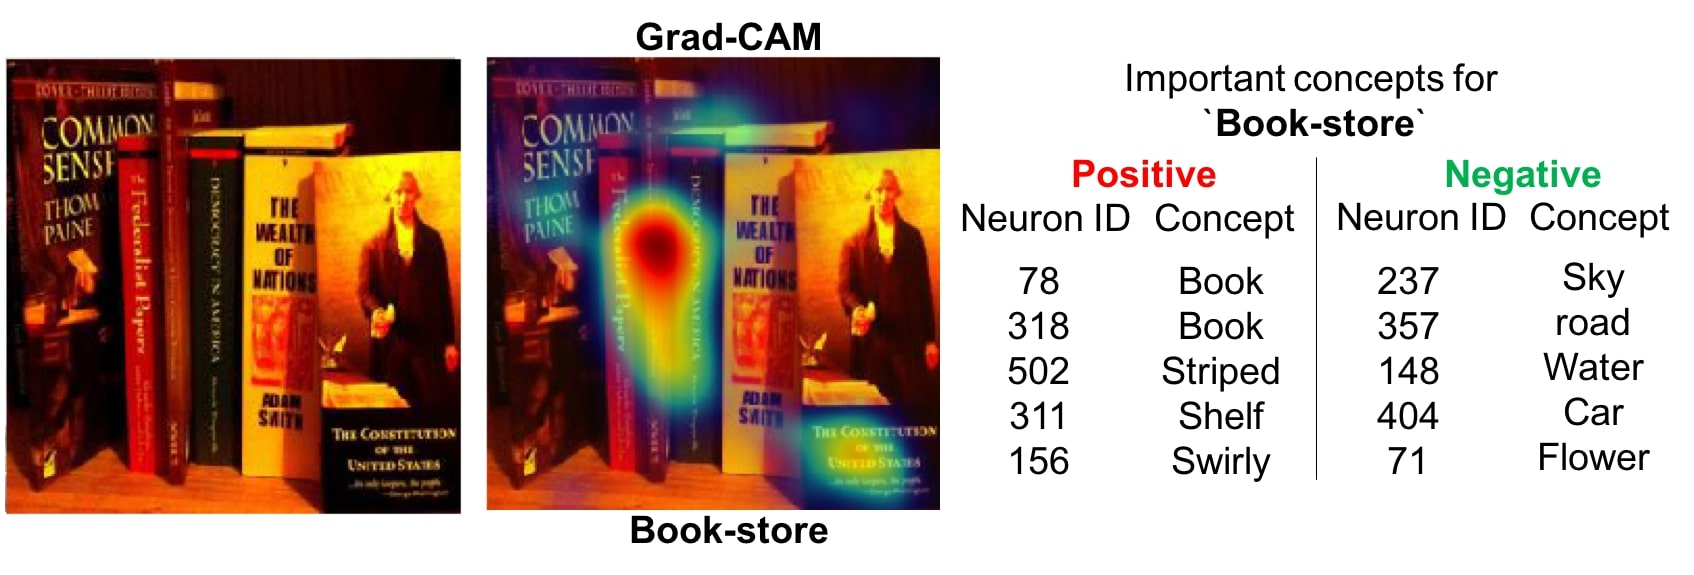
\includegraphics[scale=0.135]{figures/1_pos.jpg}\caption{}
\vspace{10pt}
\end{subfigure}
\begin{subfigure}[t]{\columnwidth}
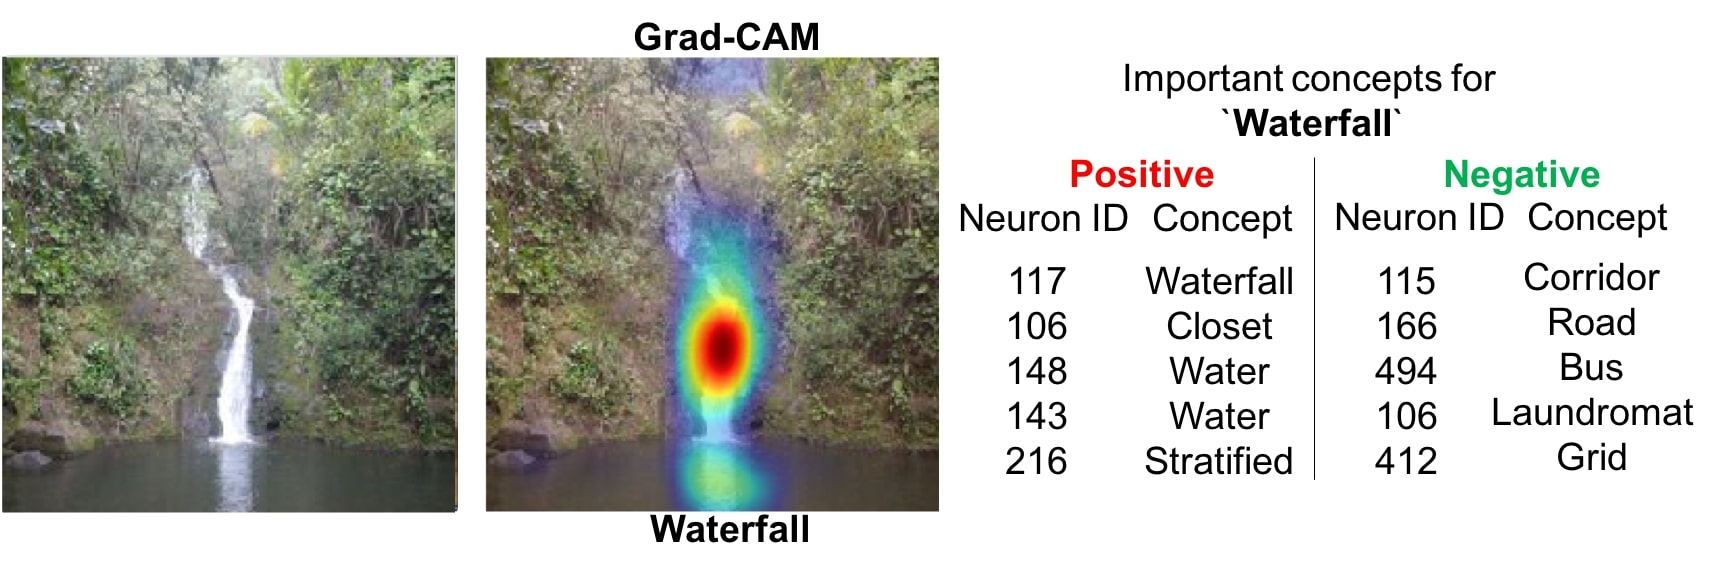
\includegraphics[scale=0.135]{figures/2_pos.jpg}\caption{}
\vspace{10pt}
\end{subfigure}
\begin{subfigure}[t]{\columnwidth}
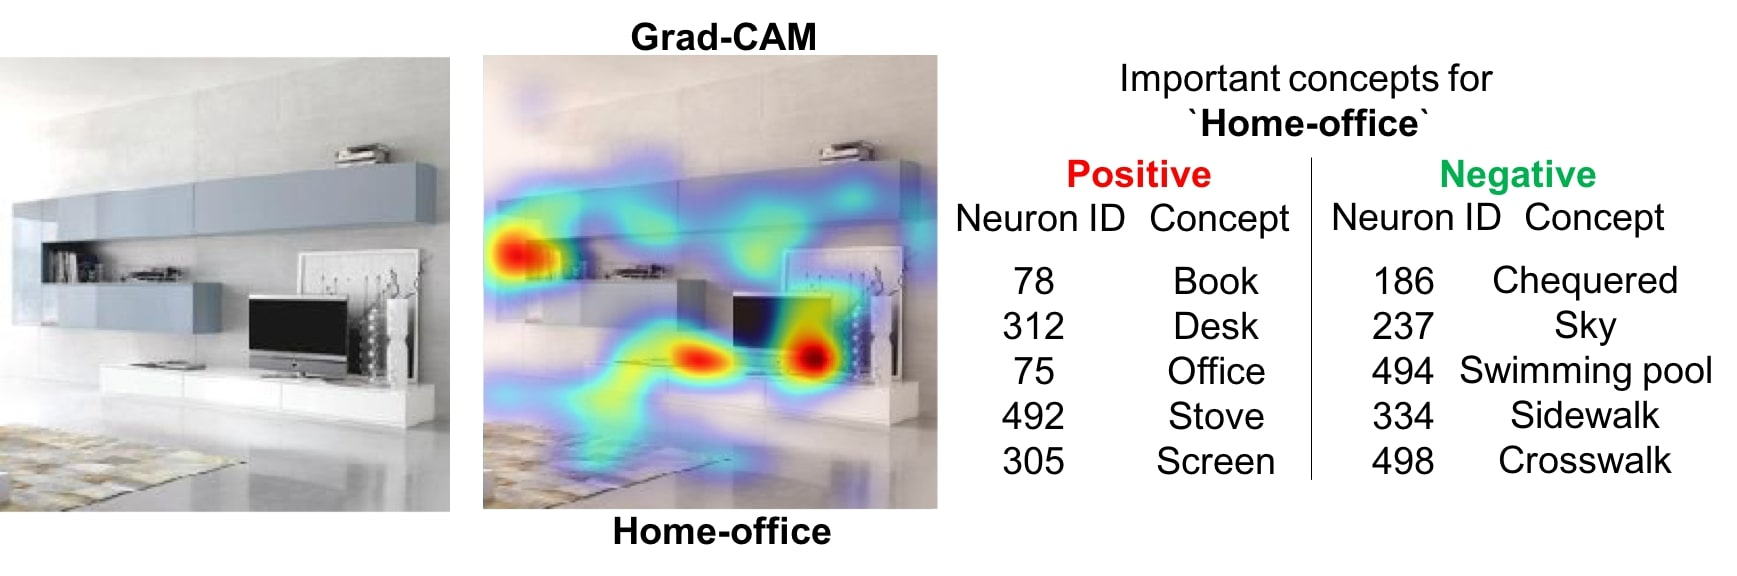
\includegraphics[scale=0.135]{figures/3_pos.jpg}\caption{}
\vspace{10pt}
\end{subfigure}
\begin{subfigure}[t]{\columnwidth}
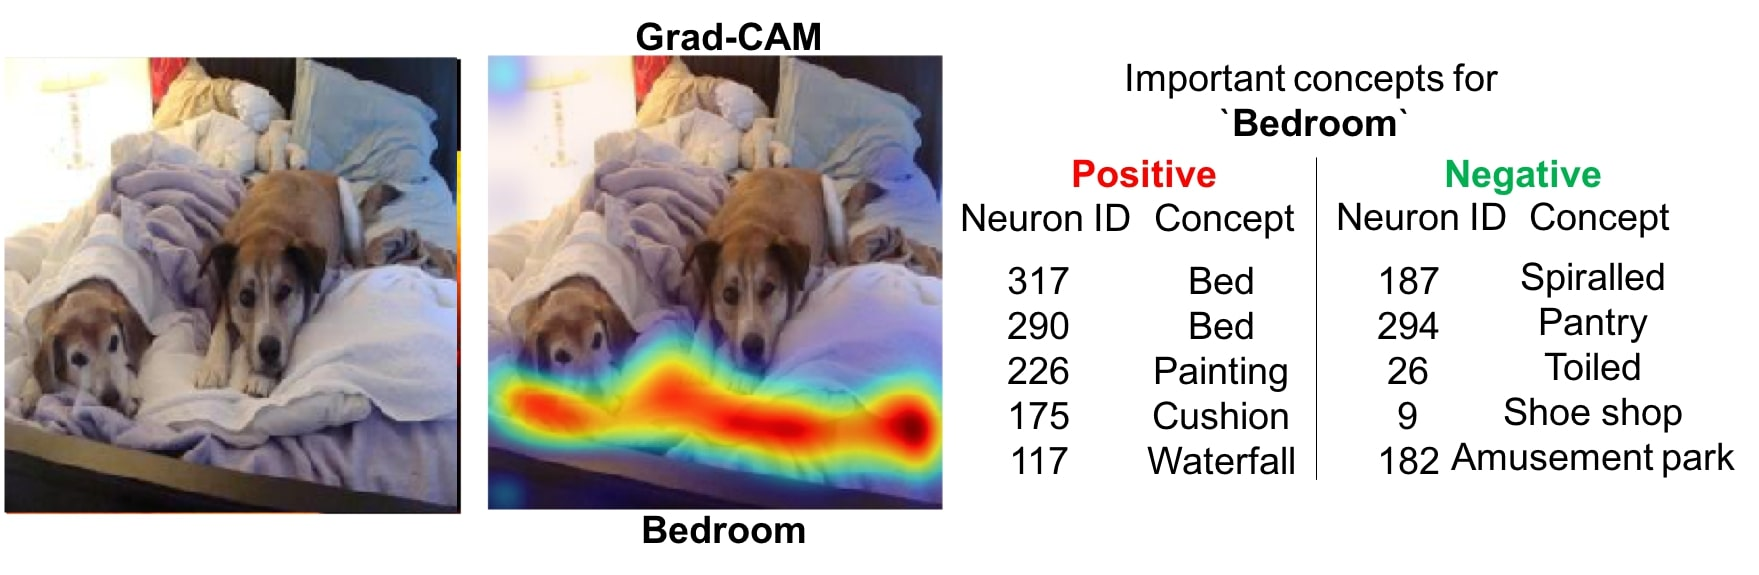
\includegraphics[scale=0.135]{figures/4_pos.jpg}\caption{}
\vspace{10pt}
\end{subfigure}
\begin{subfigure}[t]{\columnwidth}
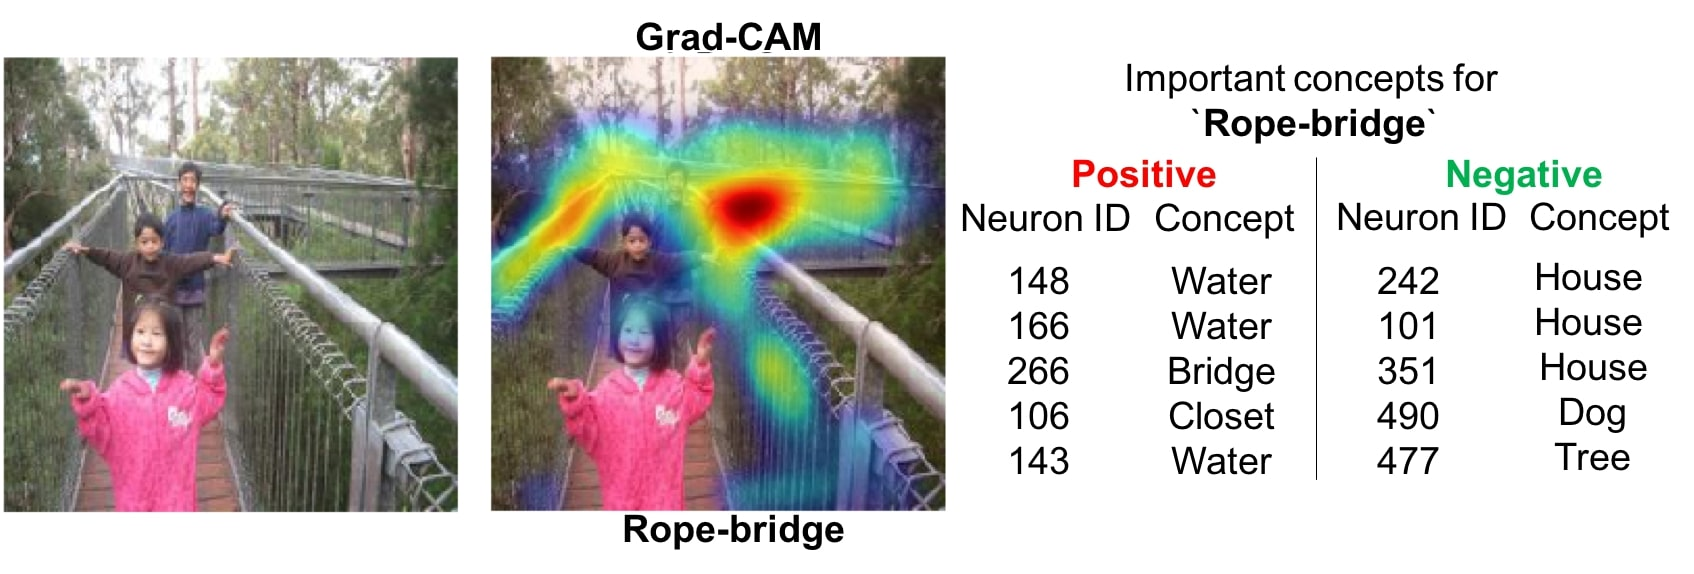
\includegraphics[scale=0.135]{figures/1_neg.jpg}\caption{}
\vspace{10pt}
\end{subfigure}
\begin{subfigure}[t]{\columnwidth}
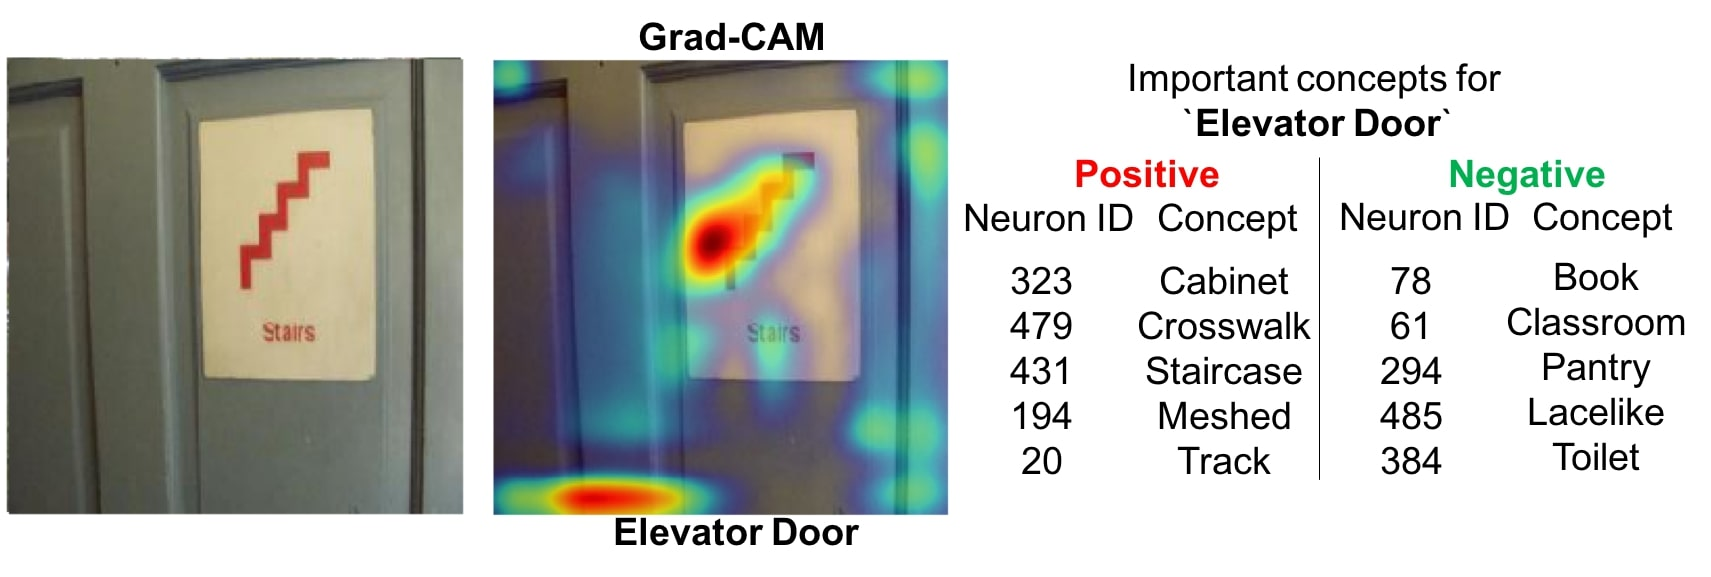
\includegraphics[scale=0.135]{figures/2_neg.jpg}\caption{}
\vspace{10pt}
\end{subfigure}
  \caption{\ijcv{Examples showing visual explanations and textual explanations for VGG-16 trained on Places365 dataset~\cite{zhou2017places}. For textual explanations we provide the most important neurons for the predicted class along with their names. Important neurons can be either be persuasive (positive importance) or inhibitive (negative importance). The first 2 rows show success cases, and the last row shows 2 failure cases. We see that in (a), the important neurons computed by \eqref{eq:alpha1} look for concepts such as book and shelf which are indicative of class `Book-store' which is fairly intuitive. %
  }}
  \label{fig:text_explanations}
\end{center}
\end{figure*}



Equation. \eqref{eq:alpha1} gives a way to obtain neuron-importance, $\alpha{}$, for each neuron in a convolutional layer for a particular class.
There have been hypotheses presented in the literature \cite{Zhou2014ObjectDE,zeiler_eccv14} that neurons act as concept `detectors'.
Higher positive values of the neuron importance indicate that the presence of that concept leads to an increase in the class score,
whereas higher negative values indicate that its absence leads to an increase in the score for the class.

Given this intuition, let's examine a way to generate textual explanations.
In recent work, Bau~\etal~\cite{netdissect} proposed an approach to automatically name
neurons in any convolutional layer of a trained network.
These names indicate concepts that the neuron looks for in an image.
Using their approach. we first obtain neuron names for the last convolutional layer. %
Next, we sort and obtain the top-5 and bottom-5 neurons based on their class-specific importance scores, $\alpha_k$.
The names for these neurons can be used as text explanations.

\reffig{fig:text_explanations} shows some examples of visual and textual explanations for the
image classification model (VGG-16) trained on the Places365 dataset~\cite{zhou2017places}.
In (a), the positively important neurons computed by \eqref{eq:alpha1} look for intuitive
concepts such as book and shelf that are indicative of the class `Book-store'.
Also note that the negatively important neurons look for concepts such as sky, road, water and car which don't occur in `Book-store' images.
In (b), for predicting `waterfall', both visual and textual explanations highlight
`water' and `stratified' which are descriptive of `waterfall' images.
(e) is a failure case due to misclassification as the network predicted
`rope-bridge' when there is no rope, but still the important concepts (water
and bridge) are indicative of the predicted class.
In (f), while \gcam{} correctly looks at the door and the staircase on the
paper to predict `Elevator door', the neurons detecting doors did not pass the
IoU threshold\footnote{Area of overlap between ground truth concept annotation and neuron activation over area of their union. More details of this metric can be found in \cite{netdissect}} of 0.05 (chosen in order to suppress the noise in the neuron names),
and hence are not part of the textual explanations. More qualitative examples
can be found in the \refsec{sec:sup_text_exp}.


